% Native editable composition from verified, unchanged IDE images.
\par
\begin{figure}[htbp]
  \centering
  \sbox0{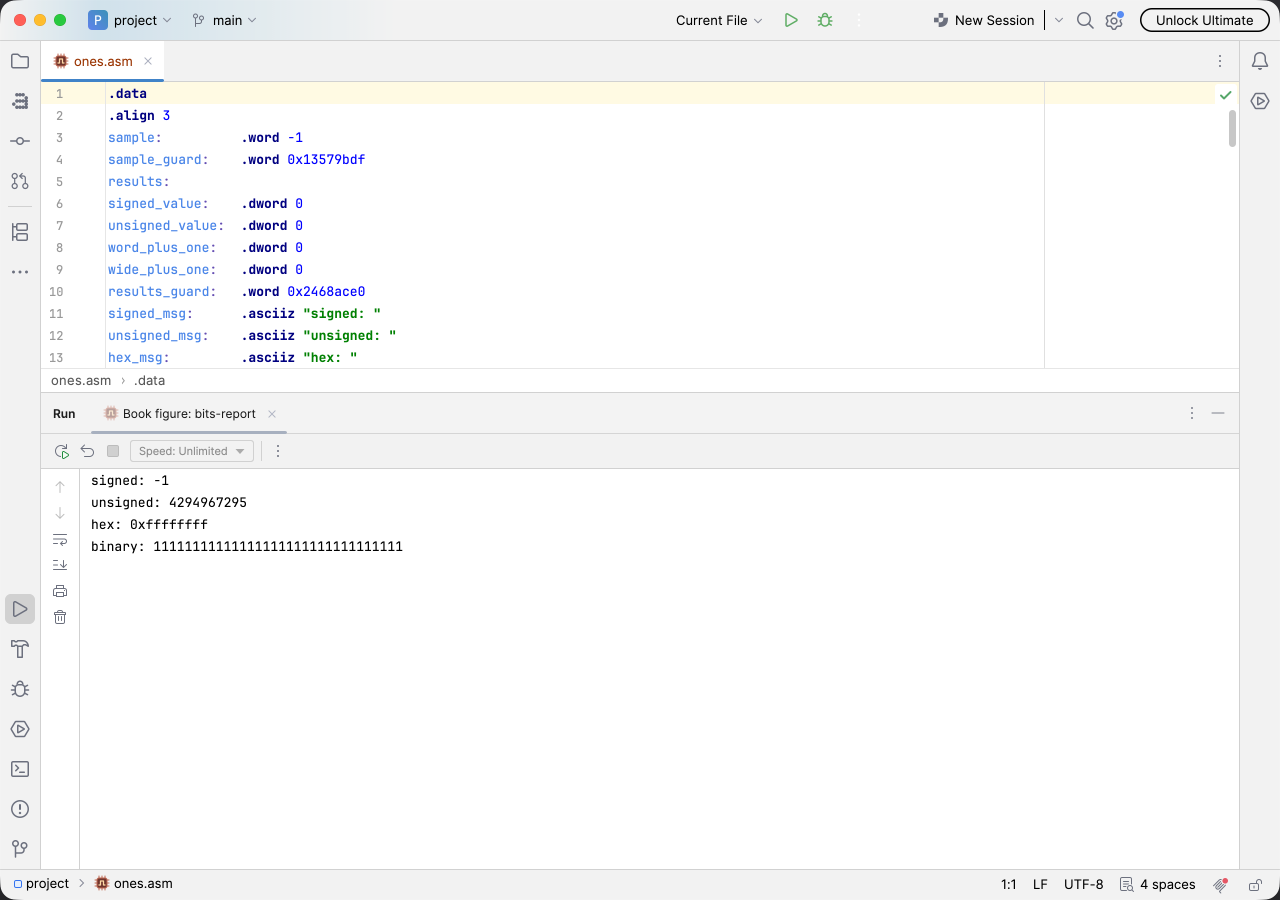
\includegraphics[artifact]{packages/004-bit-inspector/captures/f03-word-report/raw.png}}
  \edef\MARSreportdecimalLeft{\the\dimexpr0.066406250\wd0\relax}
  \edef\MARSreportdecimalBottom{\the\dimexpr0.426666667\ht0\relax}
  \edef\MARSreportdecimalRight{\the\dimexpr0.652343750\wd0\relax}
  \edef\MARSreportdecimalTop{\the\dimexpr0.517777778\ht0\relax}
  \edef\MARSreporthexLeft{\the\dimexpr0.066406250\wd0\relax}
  \edef\MARSreporthexBottom{\the\dimexpr0.402222222\ht0\relax}
  \edef\MARSreporthexRight{\the\dimexpr0.652343750\wd0\relax}
  \edef\MARSreporthexTop{\the\dimexpr0.566666667\ht0\relax}
  \edef\MARSreportbinaryLeft{\the\dimexpr0.066406250\wd0\relax}
  \edef\MARSreportbinaryBottom{\the\dimexpr0.377777778\ht0\relax}
  \edef\MARSreportbinaryRight{\the\dimexpr0.652343750\wd0\relax}
  \edef\MARSreportbinaryTop{\the\dimexpr0.591111111\ht0\relax}
  \begin{tikzpicture}[alt={Three annotated console details from a completed input-free Run. Signed decimal is minus one and unsigned decimal is 4294967295. Hexadecimal is 0xffffffff. Binary consists of exactly thirty-two one digits. The observed process exits successfully with this exact output.}]
    \node[anchor=north west,inner sep=0,font=\small\bfseries] (decimal-title) at (6mm,0) {One word, two decimal interpretations};
    \node[anchor=north west,inner sep=0] (decimal) at ([yshift=-1mm]decimal-title.south west) {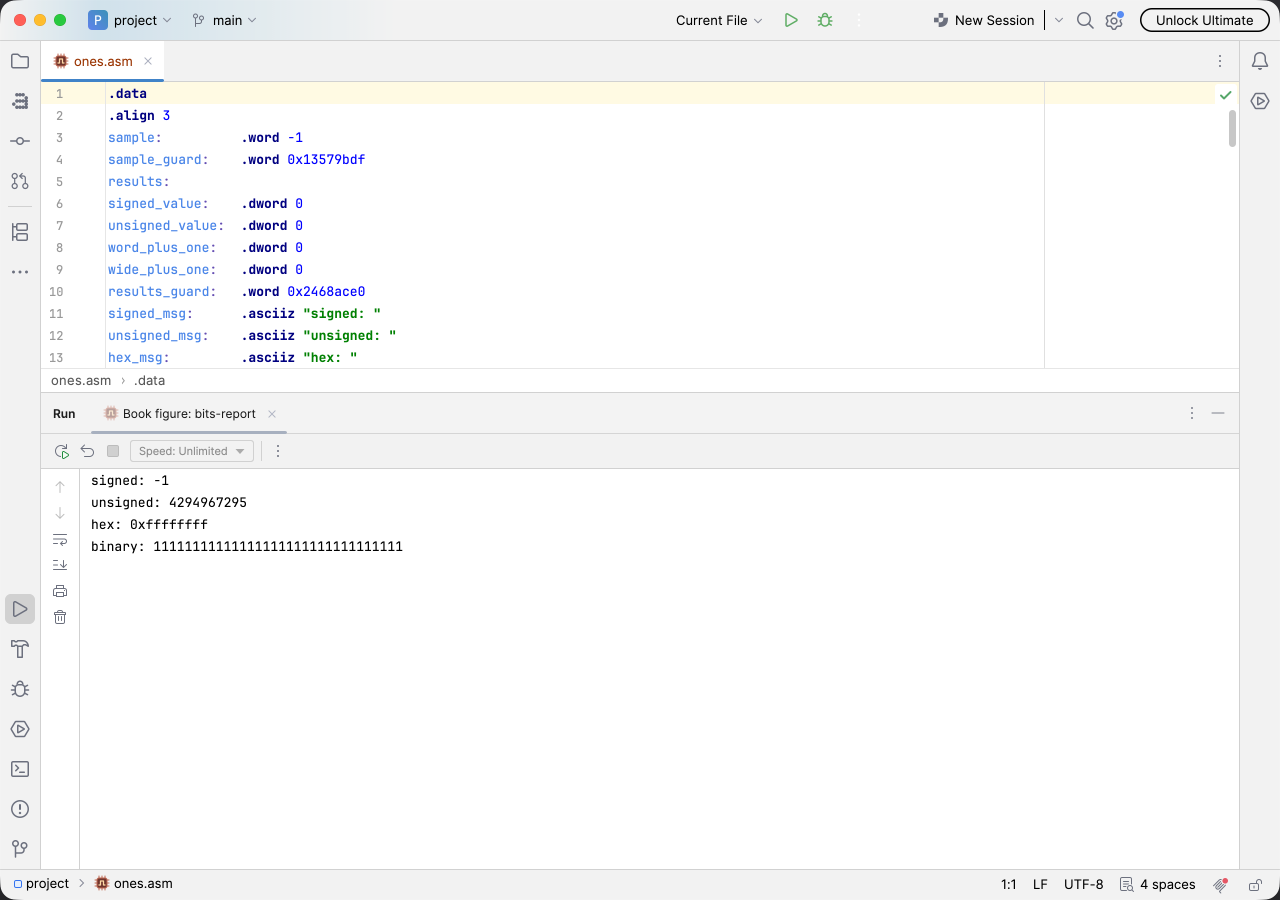
\includegraphics[width=0.7\linewidth,artifact,trim={\MARSreportdecimalLeft{} \MARSreportdecimalBottom{} \MARSreportdecimalRight{} \MARSreportdecimalTop{}},clip]{packages/004-bit-inspector/captures/f03-word-report/raw.png}};
    \begin{scope}[shift={(decimal.south west)},x={($(decimal.south east)-(decimal.south west)$)},y={($(decimal.north west)-(decimal.south west)$)}]
      \draw[black,line width=0.7pt] (0.016666667,0.060000000) rectangle (0.450000000,0.940000000);
      \node[draw=black,fill=white,circle,inner sep=1.5pt,font=\footnotesize] at ($(0.016666667,0.940000000)+(-3mm,0)$) {1};
    \end{scope}
    \node[anchor=north west,inner sep=0,font=\small\bfseries] (hex-title) at ([yshift=-2mm]decimal.south west) {Eight hexadecimal digits};
    \node[anchor=north west,inner sep=0] (hex) at ([yshift=-1mm]hex-title.south west) {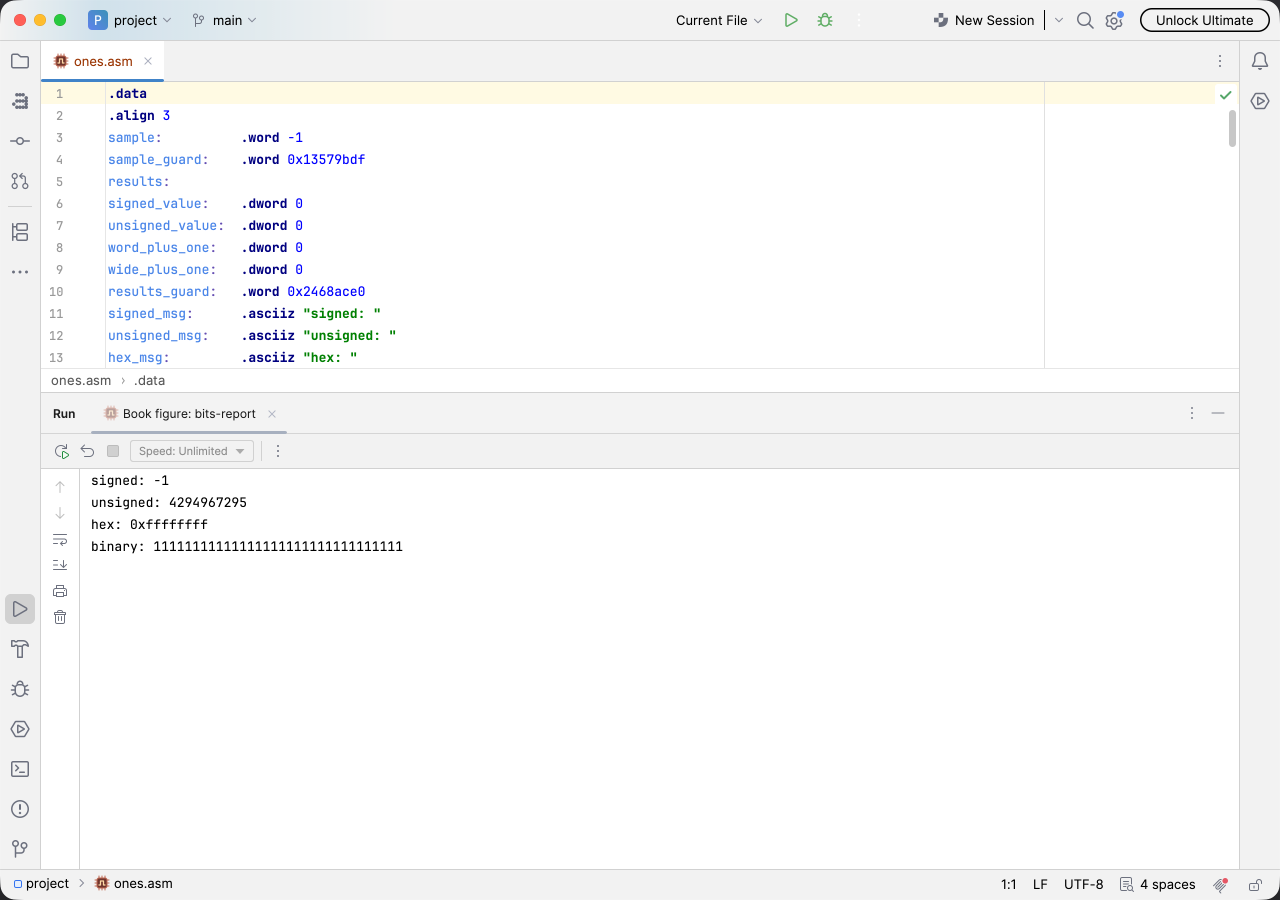
\includegraphics[width=0.7\linewidth,artifact,trim={\MARSreporthexLeft{} \MARSreporthexBottom{} \MARSreporthexRight{} \MARSreporthexTop{}},clip]{packages/004-bit-inspector/captures/f03-word-report/raw.png}};
    \begin{scope}[shift={(hex.south west)},x={($(hex.south east)-(hex.south west)$)},y={($(hex.north west)-(hex.south west)$)}]
      \draw[black,line width=0.7pt] (0.016666667,0.107142857) rectangle (0.341666667,0.892857143);
      \node[draw=black,fill=white,circle,inner sep=1.5pt,font=\footnotesize] at ($(0.016666667,0.892857143)+(-3mm,0)$) {2};
    \end{scope}
    \node[anchor=north west,inner sep=0,font=\small\bfseries] (binary-title) at ([yshift=-2mm]hex.south west) {Thirty-two binary digits};
    \node[anchor=north west,inner sep=0] (binary) at ([yshift=-1mm]binary-title.south west) {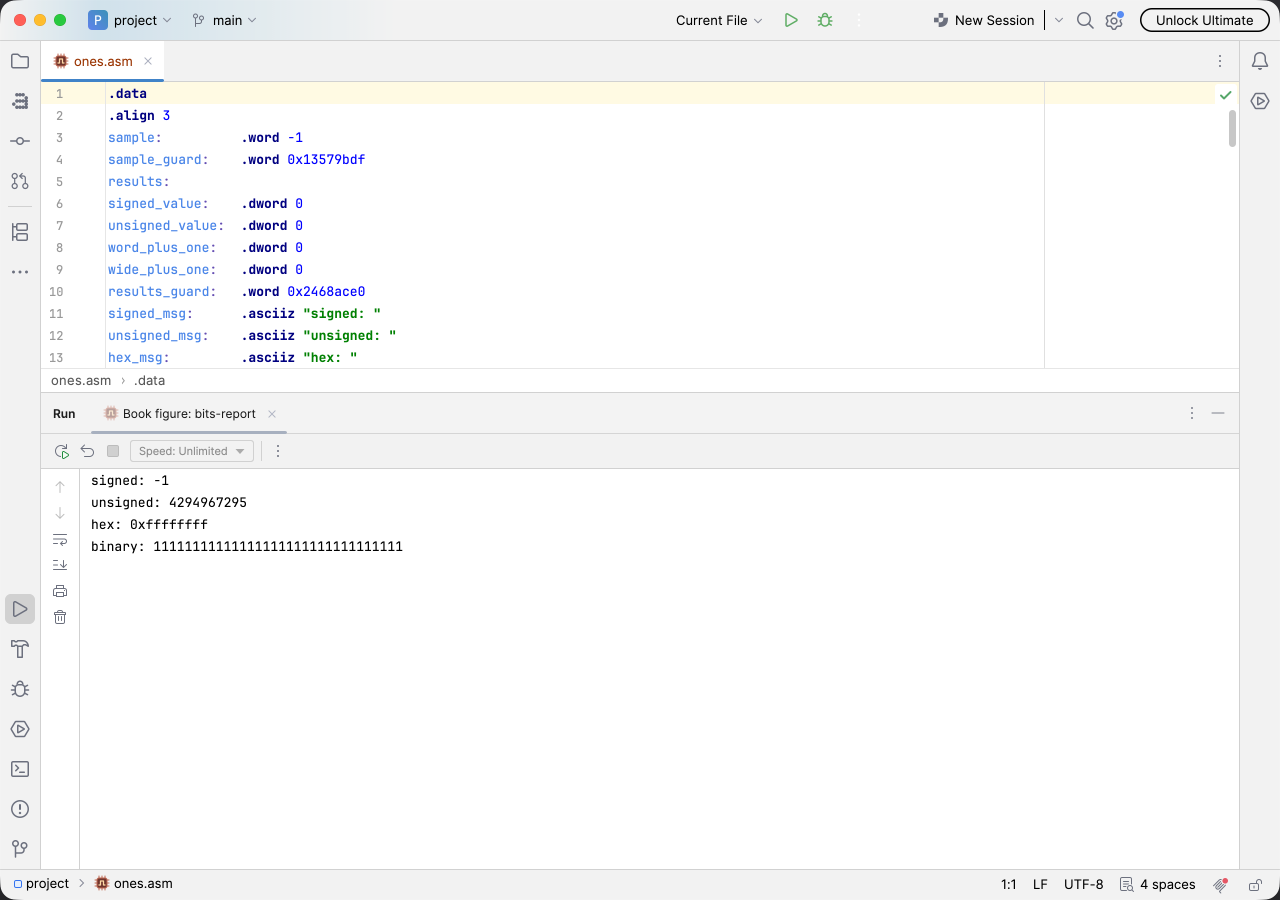
\includegraphics[width=0.7\linewidth,artifact,trim={\MARSreportbinaryLeft{} \MARSreportbinaryBottom{} \MARSreportbinaryRight{} \MARSreportbinaryTop{}},clip]{packages/004-bit-inspector/captures/f03-word-report/raw.png}};
    \begin{scope}[shift={(binary.south west)},x={($(binary.south east)-(binary.south west)$)},y={($(binary.north west)-(binary.south west)$)}]
      \draw[black,line width=0.7pt] (0.016666667,0.107142857) rectangle (0.880555556,0.892857143);
      \node[draw=black,fill=white,circle,inner sep=1.5pt,font=\footnotesize] at ($(0.016666667,0.892857143)+(-3mm,0)$) {3};
    \end{scope}
  \end{tikzpicture}
  \par\smallskip
  \begin{minipage}{\linewidth}
    \small
    \begin{enumerate}
      \item The signed and unsigned services interpret the same low 32 argument bits differently: \texttt{ffffffff} is $-1$ in signed decimal and 4294967295 in unsigned decimal. The reference supplies the preserved \texttt{\$s0} value for each format; it does not change the sample between lines.
      \item \texttt{0xffffffff} has eight hexadecimal digits, each representing four bits. This service reports a word, not all sixteen hexadecimal digits of a 64-bit register. Use the register or doubleword-memory view when the upper half matters.
      \item The binary line contains exactly 32 one digits. It presents the same word in base two. This Run ends normally after printing the newline; no prompt or input echo is part of the report.
    \end{enumerate}
  \end{minipage}
  \caption{A completed native Run prints four representations of the all-one word. This program requires no keyboard input.}
  \label{capture:004-bit-inspector-f03-word-report}
\end{figure}
\par
